%% The following is a directive for TeXShop to indicate the main file
%%!TEX root = ../diss.tex

\chapter{Oxygen-enhanced MRI}
\label{ch:oemri1}

% ======================================================================
\section{Introduction}
% ======================================================================

Hypoxia is a well-established component of the tumour microenvironment, arising most often as tumour cell proliferation outpaces the growth of new vasculature.
Tumour hypoxia is an indicator of poor prognosis and is responsible for tumour resistance to radiotherapy and some chemotherapies, but is also a potentially useful target for novel anti-cancer drugs~\cite{Wilson:2011jp}.
Assessing tumour hypoxia in the clinical setting is challenging largely due to the invasive nature of biopsy-dependent techniques and the limited capacity and high expense of the more favoured, non-invasive PET imaging of hypoxia tracers~\cite{Horsman:2012kw}.
The utility of screening patients for hypoxia was demonstrated retrospectively in trials of the hypoxic cytotoxin tirapazamine, where those patients with greater PET-imaged hypoxia experienced greater benefit~\cite{Rischin:2006fz}.
However, subsequent trials of drugs targeting hypoxia, including those for evofosfamide that failed to show clinical benefit, have not used hypoxia imaging to stratify patients.
A practical, widely applicable, and non-invasive imaging method is urgently required as a biomarker to monitor tumour hypoxia in many contexts, and is crucial to the development and clinical evaluation of future hypoxia-targeting drugs.

% this used to be the interlude
% START of the interlude
\section{Theory}
To explore the mechanism of action for the OE-MRI signal, it is useful to first understand the delivery of oxygen from inspired air to tissues. 
The primary mode of oxygen delivery to tissue is the haemoglobin (\acs{Hb}) molecule as it carries and delivers 98\% of the oxygen in the body. 
Over 250 million \acs{Hb} molecules are found in a typical red blood cell and each \acs{Hb} molecule has four binding sites for oxygen molecules. 
The binding affinity of \acs{Hb} to bind ${O_2}$ increases 

The binding affinity for ${O_2}$ drastically increases for subsequent oxygen molecules that bind to \acs{Hb} as the conformation of the \acs{Hb} molecule changes to increase binding affinity for the next oxygen, a phenomenon called cooperativity. 
Similarly, when the partial pressure of ${O_2}$ drops, the \acs{Hb} molecule changes conformation  and bound ${O_2}$ is released in a reversible process.

\subsection{Physiology}

The primary mode of oxygen delivery to tissue is the haemoglobin (\acs{Hb}) molecule as it carries and delivers 98\% of the oxygen in the body. 
Over 250 million \acs{Hb} molecules are found in a typical red blood cell and each \acs{Hb} molecule has four binding sites for oxygen molecules. 
The binding affinity for ${O_2}$ drastically increases for subsequent oxygen molecules that bind to \acs{Hb} as the conformation of the \acs{Hb} molecule changes to increase binding affinity for the next oxygen, a phenomenon called cooperativity. 
Similarly, when the local environment of the \acs{Hb} molecule changes such that O$_2$ needs to be released, the reverse conformational changes occur; a proportionately lower drop in oxygen tension is then required to release the next O$_2$ molecule. 
The dissociation of oxygen from haemoglobin molecules is well described by the oxygen-haemglobin dissociation curve (figure~\ref{HBdis}).

\begin{figure}
 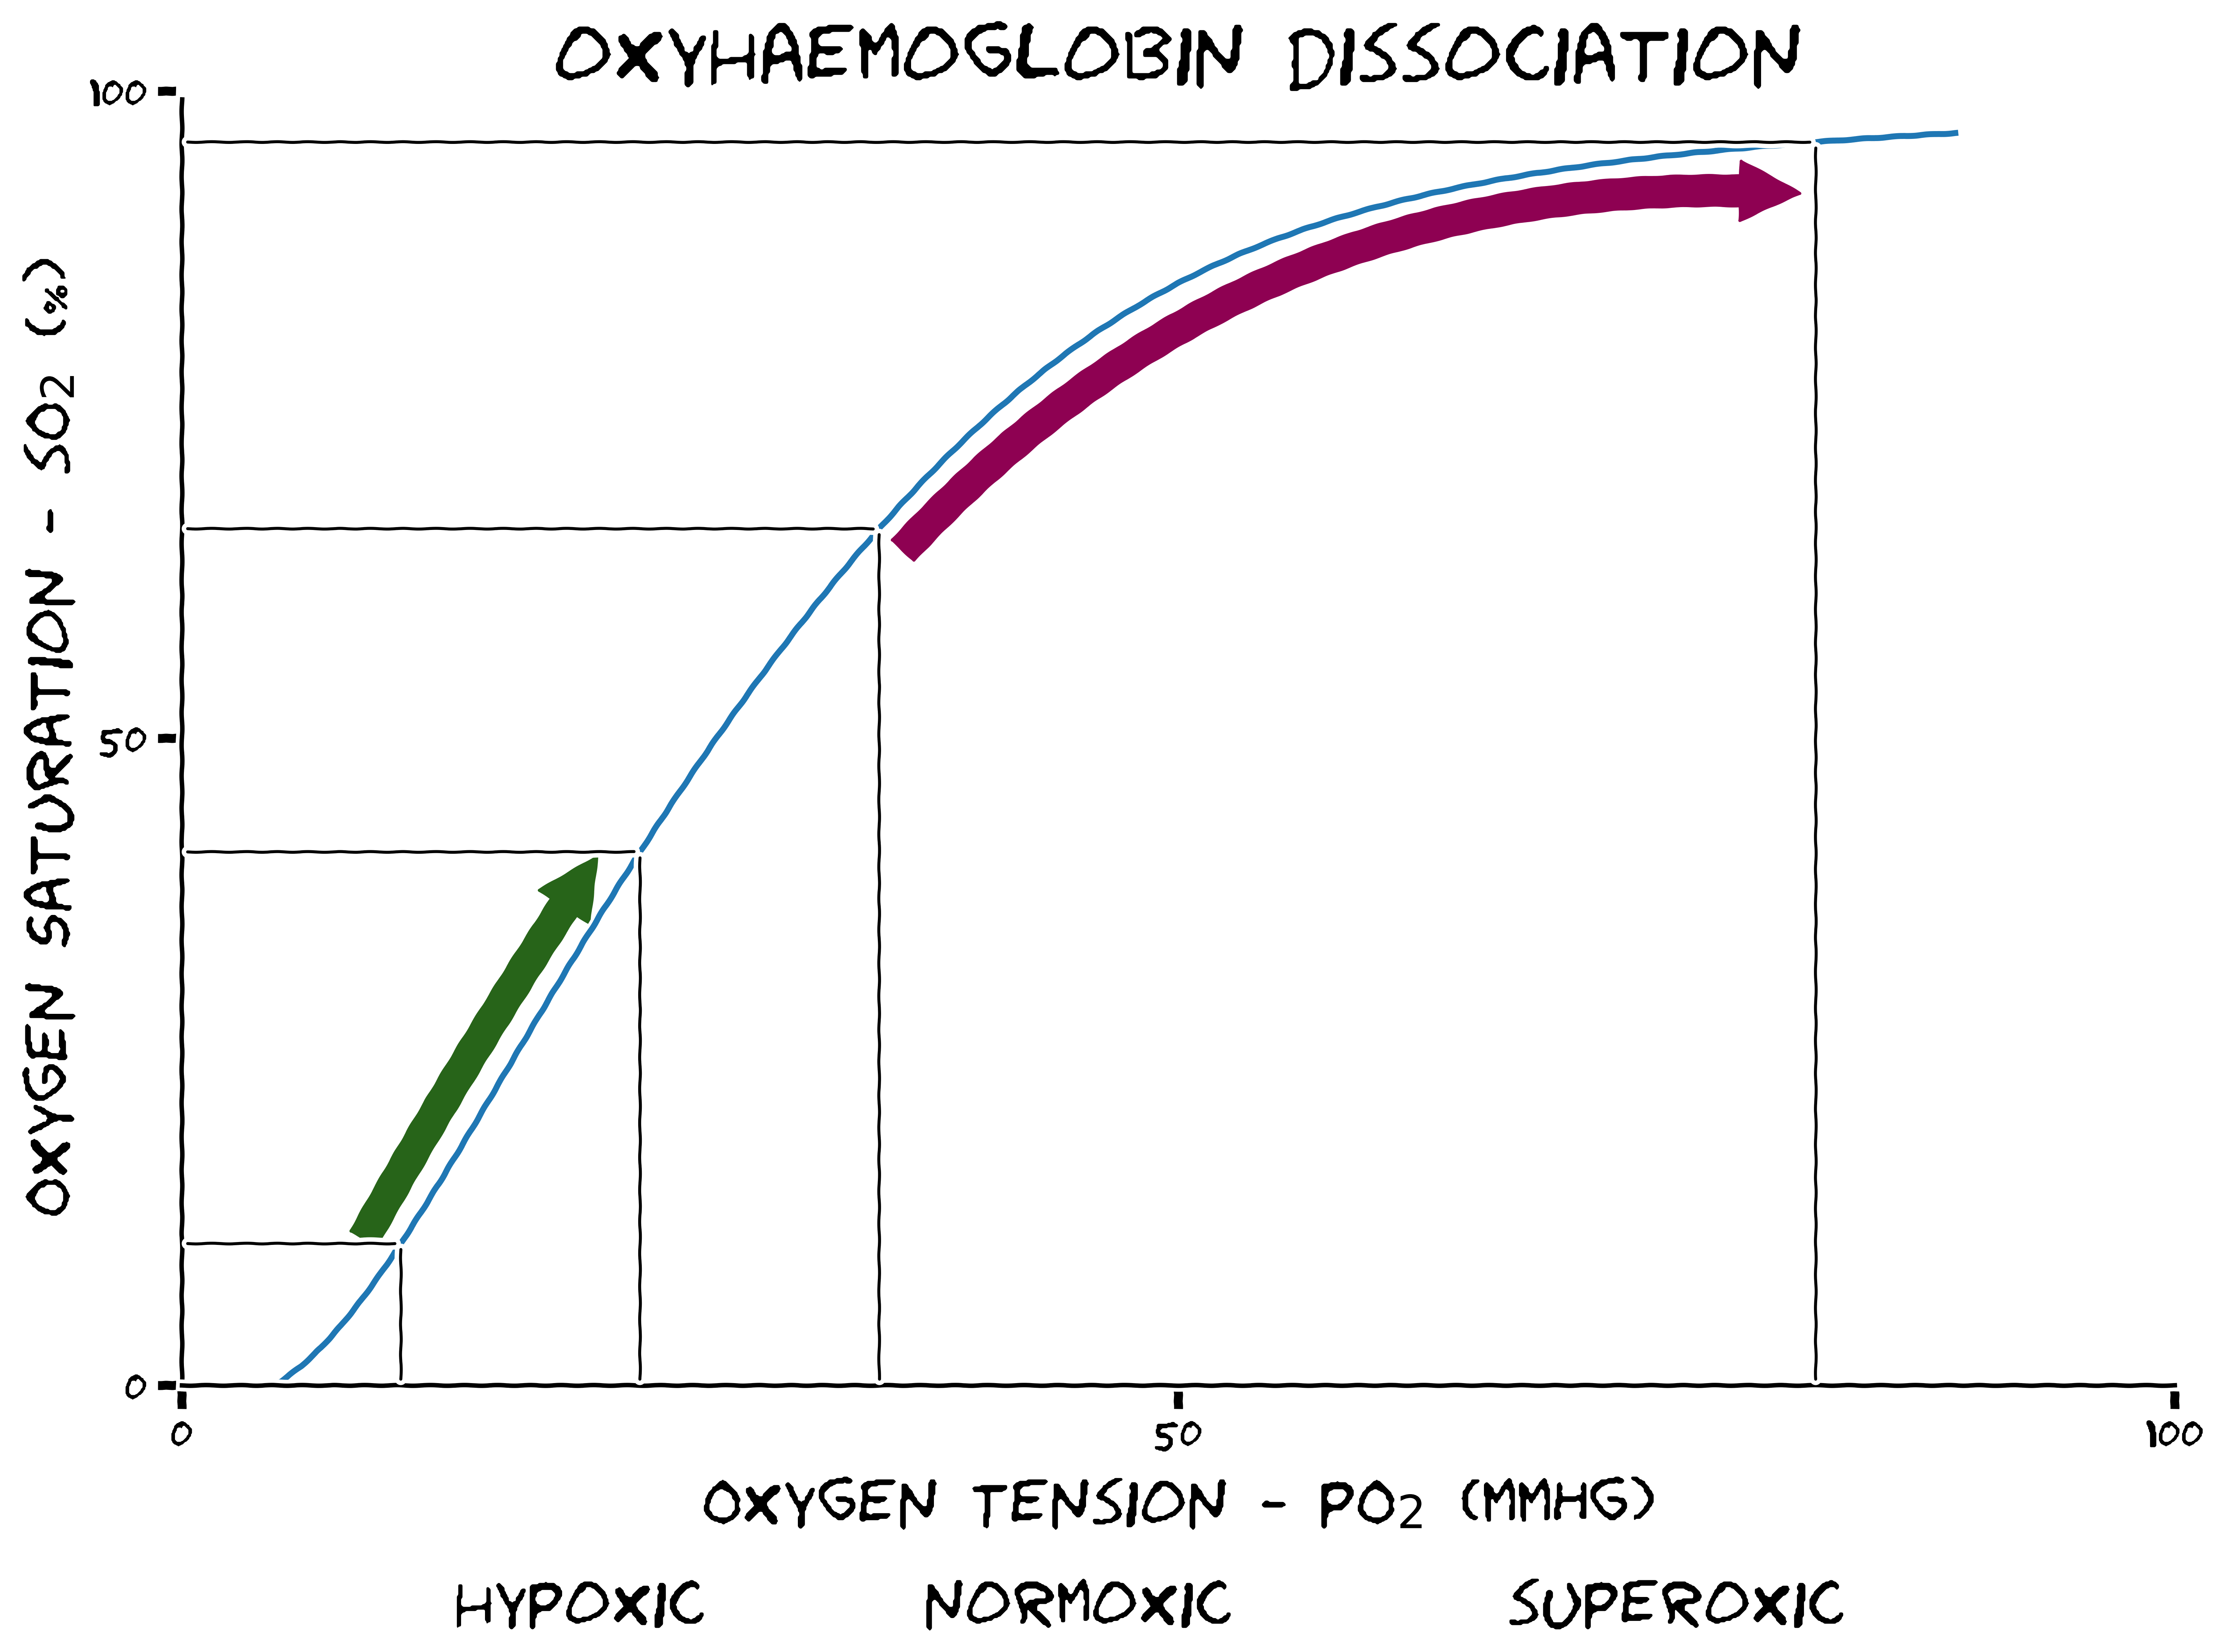
\includegraphics[width=\textwidth]{./oemri_thesis1/oemri_thesis1-images/Hbdissociation.png}
 \caption{Sigmoidal curve illustrating the relationship between the haemoglobin saturation (y-axis) and the oxygen tension (x-axis). When the oxygen tension is low, the Hb easily binds $O_2$ and there is a rapid rise in oxygen saturation (green arrow). Note that it takes a large increase in oxygen tension to bind the last O$_2$ and similarly, a large decrease in oxygen tension to release the last O$_2$ (purple arrow) ~\cite{GomezCambronero:2001hu}.}
 \label{HBdis}
\end{figure}	

Upon inspiration of atmospheric air (p$_{O_2}$ = 160 mmHg), gas exchange in the pulmonary capillary beds occurs in the alveoli of the lungs (Fig~\ref{mmhg}).
Incoming venous blood with a low oxygen tension ($p_{O_2}$ = 40 mmHg) is oxygenated as haemoglobin molecules readily bind available oxygen. 
As the oxygenated blood leaves the alveoli and moves through the systemic arteries, it has an oxygen tension of 100 mmHg. 
The oxygenated blood then travels from the arteries to the systemic capillary bed and the local oxygen tension drops from 100 to 40 mmHg.
Simultaneously, while the \acs{Hb} molecule undergoes a structural change releasing a molecule of O$_2$ from its first binding site.  
The second release of the oxygen molecule occurs when the tension drops to 26mmHg~\cite{GomezCambronero:2001hu}.
In a population of \acs{Hb} molecules fully saturated in tissue (S$_{O_2}>95\%$), the approximate $\Delta pO_2$ required to release the first ${O_2}$ molecule is 60 mmHg (100-40 mmHg).
The third ${O_2}$ molecule is released when the $pO_2$ drops from 26 to 19 mmHg, and the final ${O_2}$ molecule is released when the $pO_2$ drops to 12 mmHg~\cite{GomezCambronero:2001hu}.
Practically however, it is important to note that \acs{Hb} molecules never release all four of the bound oxygen \emph{in vivo}.
This important feature of \acs{Hb} (cooperativity) ensures that small changes in p$_{O_2}$ have the appropriate effect in the appropriate place. 
For instance, in the lung tight binding is required so \acs{Hb} can bind the O$_2$ needed to supply all the tissues.
Therefore, small changes should not affect the release of O$_2$.
Conversely, small changes in p$_{O_2}$ in capillary beds should result in quick release of O$_2$ so it can easily diffuse to oxygen-starved tissues. 

\begin{figure}
    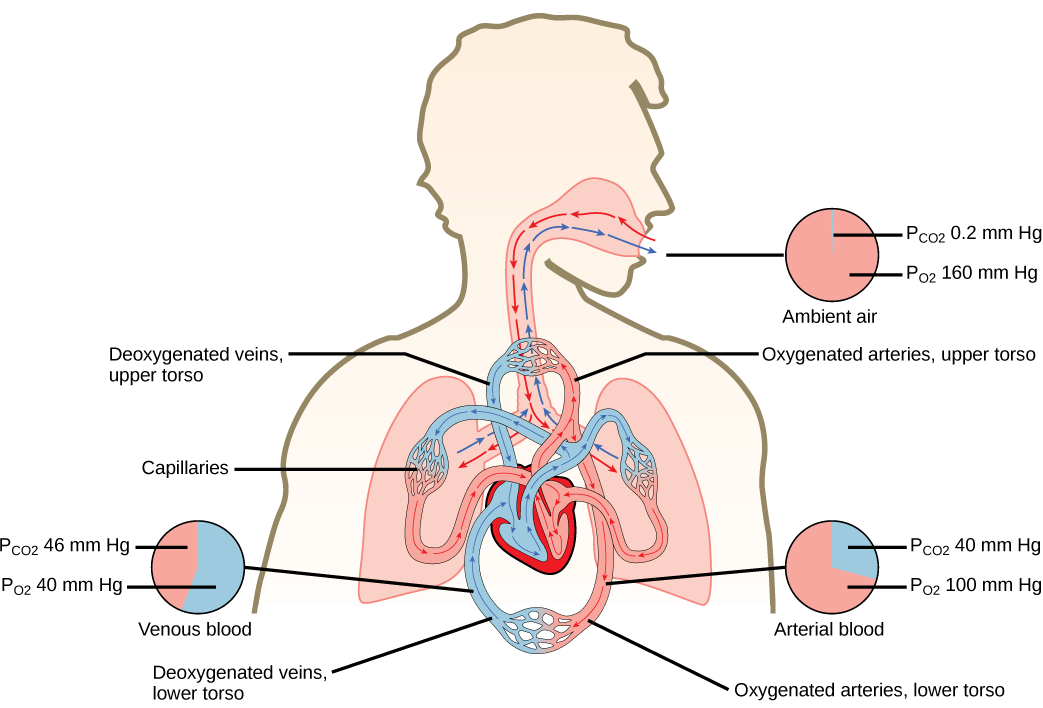
\includegraphics[width=0.8\textwidth]{./oemri_thesis1/oemri_thesis1-images/mmHg.png}
    \caption{A schematic of the change in the partial pressures of oxygen and carbon dioxide at various points in the body.
    The $p_{O_2}$ of inhaled ambient air is 160 mmHg, and this is breathed in to the lungs.
    Oxygen diffuses out of the alveoli into the surrounding capillaries and binds to Hb due to the pressure gradient (capillary $p_{O_2}$ is 40 mmHg).
    This oxygenated blood ($p_{O_2}$ = 100mmHg) now enters the heart and is pumped through the body, with the Hb releasing oxygen through capillaries due again to the pressure gradient (tissue $p_{O_2}$ is $<$ 40 mmHg)~\cite{OpenStaxBio:2016uu}. 
    Textbook content produced by OpenStax Biology is licensed under a \href{https://creativecommons.org/licenses/by/4.0/}{CC-BY 4.0 license}}
    \label{mmhg}
\end{figure}

\subsection{Origin of the OE-MRI Signal}

Oxygen is a paramagnetic molecule because it has two unpaired electrons and it is widely reported that the dominating effect in the OE-MRI signal is a T$_1$ decrease after concentrated oxygen gas (100\% O$_2$) is breathed in~\cite{OConnor:2016ee,Linnik:2013hf}. 
The excess oxygen travels through the blood stream dissolved in plasma and diffuses through the vessel walls and dissolves in interstitial tissue fluid (figure~\ref{oemri}).
The net increase in dissolved oxygen results in a dramatic and measurable decrease in T$_1$. 
This change is reversed soon after the patient is switched back to breathing atmospheric air as excess oxygen is expelled or metabolized. 
Perfused tumour regions (i.e regions that already have a high \acs{Hb}-O$_2$ saturation) will see a measurable decrease in T$_1$. 
The perfused regions that do not show a decrease in T$_1$ must therefore be hypoxic~\cite{OConnor:2016ee}. 
Importantly, OE-MRI does not yield any information about unperfused regions and in that region, there are likely to be pockets of viable (but hypoxic) tissue.

The oxygen status of healthy tissue is fairly well regulated in normal tissue and every cell in the body is at most 150$\mu$m away from a blood vessel. 
In tumours however, the vascular network is chaotic and the growth patterns of vessels are abnormal leading to a defective and leaky endothelium~\cite{McDonald:2002ut}. 
Irregular diameters of tumour vessels, abnormal branching patterns and porous vessel walls all contribute to an increase in vessel permeability and pockets of hypoxic tissue. 
While $O_2$ tension is by far the largest factor in determining Hb staturation, the oxygen status in tumours is not well characterized due to the dysregulated physiological factors such as temperature, pH, and carbon dioxide concentration. 
Furthermore, these hypoxic regions are heterogeneous, transient, and drastically differ between tumour models. 
In a mammary adenocarcinoma mouse tumour model, Sorg et al. used spectral imaging with an implanted window chamber to show that upon breathing 100\% oxygen, the \acs{Hb} saturation in the tumour vascular network increases from 20-30\% up to 70-80\% while the \acs{Hb} saturation in the normal vascular network does not change appreciably~\cite{Sorg:2008eg}.

\begin{figure}
	\begin{center}
	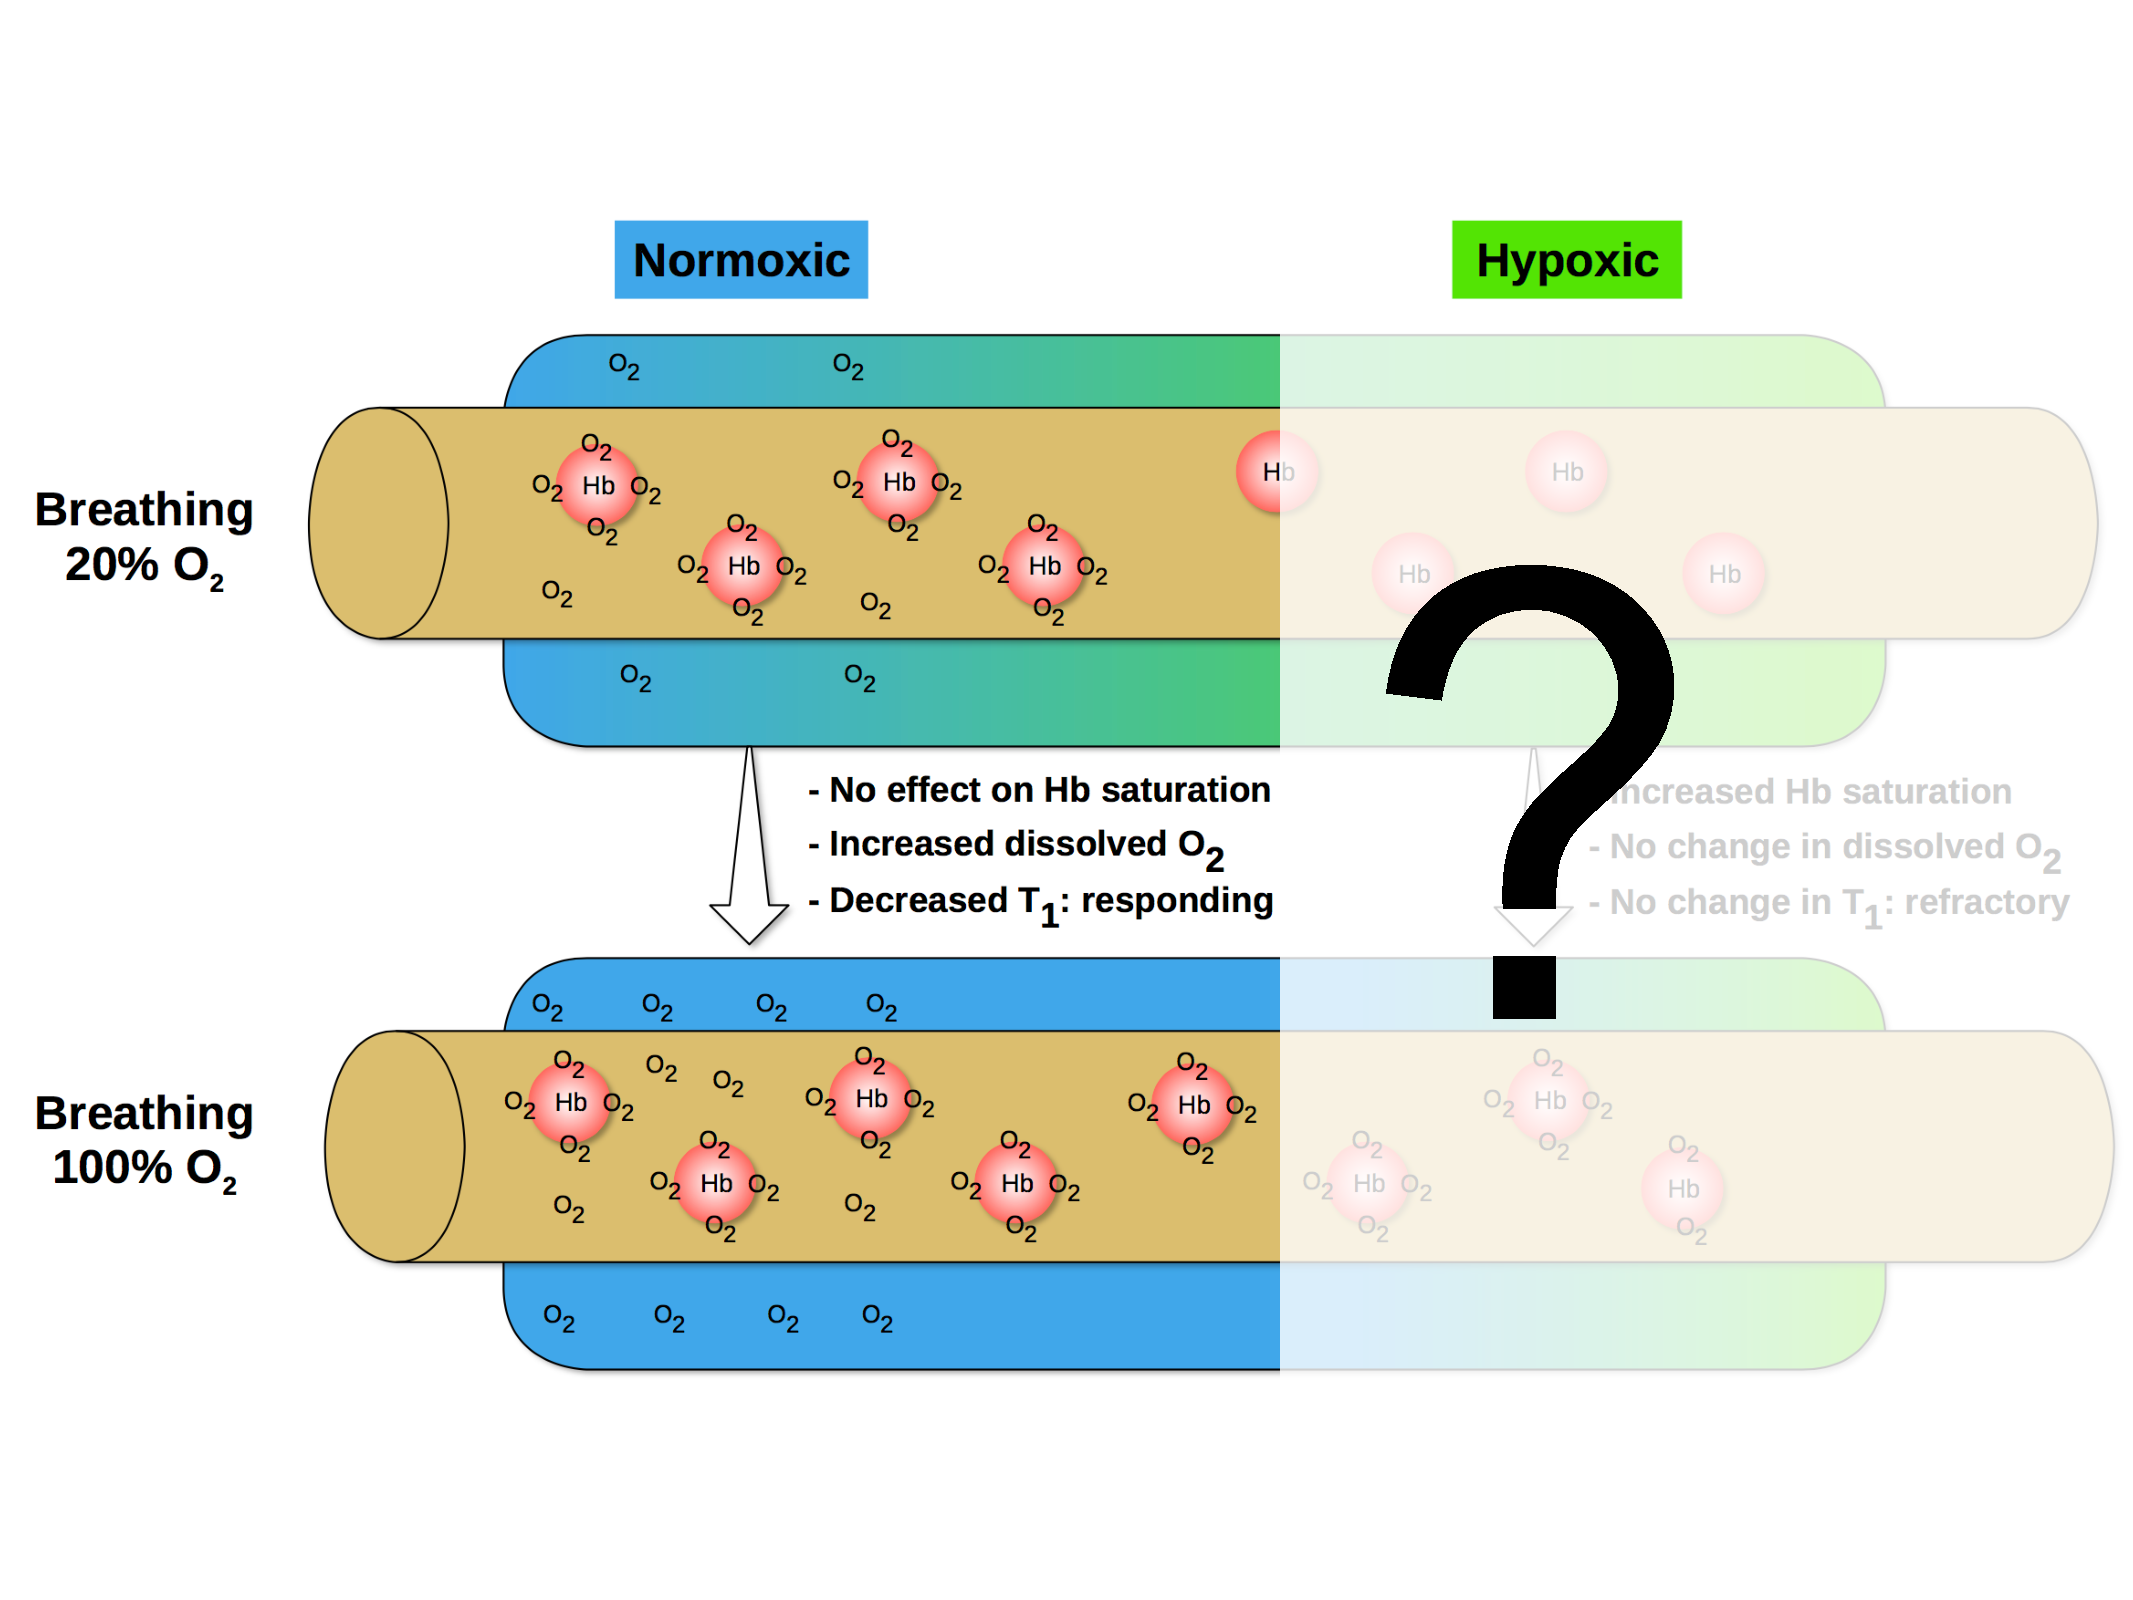
\includegraphics[width=\textwidth]{./oemri_thesis1/oemri_thesis1-images/oemriDark.pdf}
	\caption{A schematic representation of the origin of the OEMRI effect. In normoxic tissue, \acs{Hb} is almost fully saturated and any excess breathed O$_2$ cannot bind to the \acs{Hb} molecule. Consequently, O$_2$ dissolves in the blood plasma and as the excess oxygen diffuses out into the tissue, it also dissolves in the interstitial tissue fluid resulting in a net T$_1$ decrease. It is hypothesized that in the hypoxic tissue, \acs{Hb} is not fully saturated with oxygen due to increased tissue demands and/or a poorly organized vascular network. The excess breathed oxygen in this case binds to the \acs{Hb} molecule and does \textbf{not} dissolve in the plasma leading to no change in T$_1$.}
	\label{oemri}
	\end{center}
\end{figure}
% End of the interlude

\section{Motivation}

The T$_1$-shortening property of oxygen dissolved in fluid has been known since 1955~\cite{Chiarotti:1955kf} and pioneering work by Young et al. showed that oxygen acts as a paramagnetic contrast agent by demonstrating its ability to reduce T$_1$ upon inhalation~\cite{Young:1981vf}. 
Inhalation of 100\% oxygen has also been shown to elicit strong T$_1$ effects in the kidney\cite{Jones:2002dh}, spleen\cite{Tadamura:1997vc} and the poorly oxygenated retina~\cite{Berkowitz:2001uz}. 
Subsequent oxygen-enhanced MRI (OE-MRI) efforts have included either acquisition of quantitative T$_1$ maps before and after oxygen breathing, or acquiring dynamic T$_1$-weighted (T1W) signal intensity images and calculating $\Delta$T$_1$ during periods of oxygen inhalation.
The subtle but measurable influence of tissue oxygenation on T$_1$ in tumours has been reported by O'Connor~\cite{OConnor:2016ee,OConnor:2009ku,OConnor:2009bp,Little:2018iu}, Mason~\cite{Zhao:2015ez,White:2016fz,Hallac:2014cb}, Gallez~\cite{Jordan:2012do}, and others~\cite{Tadamura:1997vc,McGrath:2008kx,Kershaw:2010ha,Linnik:2013hf}. 
However, due to the changes in T$_1$ that arise as oxygen dissolves in the plasma and interstitial fluid being quite small, T$_1$ maps have poor sensitivity and application of OE-MRI techniques in cancer has yielded mixed success.
OE-MRI continues to suffer from low \acs{SNR} and it has not found routine clinical use largely because isolating small signal changes due to dissolved O$_2$ is a challenge~\cite{OConnor:2016ee, Zhao:2015ez}.

Typical imaging times for existing OE-MRI methods range from 20-45 minutes often making it impractical for easy inclusion in experimental protocols. 
An MRI technique measuring tumour oxygenation that is sensitive, fast, flexible, repeatable, and non-invasive has the potential to significantly impact the clinical fields of radiation biology and hypoxia drug targeting.
In this study, we present a new dynamic OE-MRI (dOE-MRI) method that allows extraction of very small dynamic signal changes in T$_1$W images by inducing step changes in the inspired oxygen through a repeated, cycling gas challenge.
To isolate the signal component that matches cycling gas, a machine-learning approach called independent component analysis (\acs{ICA}) is used to analyze MR images as first proposed by McKeown at al~\cite{McKeown:1998wo}.
\acs{ICA} is a form of blind source separation algorithm that separates the additive signals on the basis of the statistical independence of individual components~\cite{Hyvarinen:2000vk}.
With the application of a cycling oxygen challenge and processing the data using \acs{ICA}, our \acs{dOE-MRI} approach represents a significant improvement in the sensitivity and application of MRI for measuring tumour oxygenation, making it more practical for wide application.
% ======================================================================
\section{Methods}
% ======================================================================
\subsection{Mice and tumours}

 
Female NRG mice were implanted with murine squamous cell carcinoma SCCVII tumours ($5 \times 10^5 $cells in 50~$\mu$l serum-free media; cells provided by Dr.\ J Evans) or with human colorectal carcinoma HCT-116, human ovarian carcinoma SKOV3 or human breast carcinoma BT-474 tumours (each as $10 \times 10^6$ cells in 50~$\mu$l serum-free media; cell lines obtained from the American Type Culture Collection) and were imaged when the largest tumour diameters reached approximately 8-10~mm.
Mice were anesthetized with isoflurane for the duration of imaging sessions until euthanasia, and were positioned supine on the custom surface coil apparatus.
Throughout the imaging session, a small animal monitoring system (SA Instruments Inc., Stony Brook, NY, USA) was used to monitor respiration rate, varying between 80-100 breaths per minute, and body temperature, maintained at $36.8 \pm 0.5^\circ$C using a continuous airflow heater.
All animals were injected with 60~mg/kg pimonidazole hydrochloride (HypoxyProbe) 30~min prior to imaging to label hypoxic cells and were euthanized within 15~min of imaging completion.
Tumours were embedded and frozen in optimum cutting temperature medium (OCT; Tissue-TEK).

%\subsection{Immunohistochemistry, image acquisition and analysis}
%Co-planar MRI slices and histological sections were obtained by imaging perpendicular to the longest tumour axis in MRI and serial-step 10 $\mu m$ cryosections were cut at 0.5-mm intervals in the same plane.
%Slides were then fixed in acetone-methanol for 10-min and whole sections were immunohistochemically stained~\cite{Kalra:2017is} for CD31 (PECAM; visualized using secondaries labeled with Alexa 647nm) to label blood vessels, and for pimonidazole (HypoxyProbe-1; visualized using secondary labeled with Alexa 546nm) to label hypoxic cells. Sections were then stained using Hoechst 33342 (bisbenzimide) to label all cell nuclei.
%Whole-tumour sections were imaged using a robotic fluorescence microscope (Zeiss Axioimager Z1), a cooled, monochrome CCD camera (Retiga 4000R; QImaging), a motorized slide loader and x-y stage (Ludl Electronic Products) and customized ImageJ software~\cite{Collins:2007jr}. 
%Adjacent microscope fields of view were tiled such that images of entire tumour cryosections were captured at a resolution of 1.5 $\mu m$/pixel. 
%Using anatomical landmarks and accumulated thicknesses of serial-step sections as estimates of distances from the edges of whole tumours, sections were chosen to match the MR slices. 
%ImageJ and user-supplied algorithms were used to super impose digital images which were then manually cropped to tumour tissue boundaries with staining artifacts removed. A threshold was applied to images to identify positive pimonidazole staining, and the number of positive pixels was determined as a percentage of the total number of pixels in the tumour image. The histological hypoxic fraction is reported in the highly necrotic HCT-116 tumours as the percentage of pimonidazole+ pixels summed with the percentage of necrotic pixels, as this value should most closely approximate the MR imaging data that does not discriminate between these regions; SCCVII tumours do not have necrosis and so the same value is reported as the percentage of pimonidazole+ pixels.
%Overlaid greyscale images were converted to false color for visualization with pimonidazole as green and CD31 as magenta. 

\subsection{MRI Data Acquisition}
\label{doemri_mrianalysis1}
All MRI experiments were performed at the UBC MRI Research Centre on a 7T Bruker BioSpec 70/30 scanner at room temperature with a volume transmit coil and custom surface receive coil.
Each imaging session began with pilot axial and coronal T$_2$-W scans for tumour localization and slice prescription.
Eight contiguous axial slices (1~mm thickness) were acquired with an in-plane field of view of 3.84~cm$\times$1.92~cm and a matrix size of 128$\times$64.
Dynamic oxygen-enhanced MRI (dOE-MRI) scans were acquired with a 2D multi-slice FLASH-based sequence with T$_E$/T$_R$ = 2.67/66.7, $\alpha=40^\circ$, temporal resolution of 4.3~s with 198 repetitions for a total scan time of about 14~min.
The spatial resolution and geometry for all scans in the imaging session were matched and an experienced operator outlined the tumour on each slice of the anatomy MR images to construct the region of interest (ROI) for each animal.

\noindent\textbf{Gas challenge during MRI:} tumour-bearing mice began the \acs{dOE-MRI} gas challenge breathing medical air and were switched between 100\% oxygen and medical air in two-minute intervals.
This paradigm continued for three cycles over a total of fourteen minutes; gases were switched manually and each switch took about five seconds to complete.

\subsection{MRI Data Analysis}
\label{doemri_mrianalysis2}
\textbf{dOE-MRI maps:} A suite of in-house software was developed based on the technique described by Hyvarinen~\cite{Hyvarinen:2000vk}.
Specifically the python machine learning library scikit-learn, \texttt{sklearn.decomposition.FastICA}, was used~\cite{Pedregosa:2011tv}.
The Fast\acs{ICA} algorithm is applied to serially acquired T$_1$W images and the output is a paired set of components and weighting factors for each voxel in the dataset.
Extracted independent components are not ordered and while the component selection can be automated, in this study an observer was assigned to select the appropriate component (Figure~\ref{technique}).
The number of independent components for each imaging session was chosen by the operator and ranged from 4-9 to ensure the cyclic behaviour of the T$_1$W signal intensity corresponding to the gas challenge appeared in only one component. 
The \acs{dOE-MRI} maps were obtained by dividing the \acs{ICA} weighting-factor maps by the mean signal-intensity maps to obtain a spatial map for the strength of a particular voxel's contribution to the component of interest ($c_4$ in Figure~\ref{technique}).
In these \acs{dOE-MRI} maps, voxels are coloured to indicate the amount by which a given pixel intensity timecourse is modulated by the oxygen-related component.  
The green-white-purple colour spectrum depicts the degree to which voxels respond to the cycled gas challenge.
Purple indicates O$_2$-positive voxels whose timecourse exhibits a higher and more positive contribution from the corresponding \acs{ICA} component, representing an increase in T$_1$W signal intensity in response to the supplied 100 \% oxygen, and corresponding to areas with excess dissolved oxygen. 
O$_2$-negative voxels that show a decrease in T$_1$W signal intensity with a negative contribution from the corresponding \acs{ICA} component under 100 \% oxygen breathing are depicted as green. 
Regions whose T$_1$W signal intensity timecourses responds only weakly or not at all to the gas challenge are shown in white hues.
Fraction of voxels that are negative on \acs{dOE-MRI} maps were correlated with the histological hypoxic fraction using Pearson's r.

\noindent\textbf{OE-MRI without \acs{ICA}:} To assess whether or not \acs{ICA} was necessary to create oxygenation maps, the MR signal intensity data was correlated with two modeled paradigms: 1) a square wave which corresponds to the concentration of delivered oxygen; 2) a synthetic hemodynamic response function (HDRF) created by convolving a square wave with an exponential ($\tau=0.32$ms).
Correlations were calculated voxel by voxel using:

\begin{equation}
r = \frac{\Sigma^n_{i=1} (x_i - \bar{x}) (y_i - \bar{y})}{\sqrt{\Sigma^n_{i=1} (x_i - \bar{x})^2 \Sigma^n_{i=1} (y_i - \bar{y})^2}}
\end{equation}
where $x$ is the model paradigm and $y$ is the T$_1$W signal intensity timecourse.
The resulting correlation maps are estimates of the strength of the input paradigms with the acquired signal intensity.

% ======================================================================
\section{Results}
% ======================================================================

\subsection{\texorpdfstring{\acs{ICA}}{ICA} isolates small changes in \texorpdfstring{T$_1$}{T1}W signal intensity}

An example signal intensity vs.\ time curve is shown for a whole slice ROI compared with a single voxel (Figure~\ref{technique}B).
A mean signal intensity increase is seen for both the whole slice and the individual voxel during each of the oxygen periods of the cycle, however the magnitude of $\Delta SI$ for the individual voxel is about 10\% and the noise is of the same order of magnitude.
The slice-averaged timecourse has much less noise compared to the individual voxel, but the size of the effect is significantly reduced, the contrast to noise is similarly poor, and all spatial heterogeneity in the response is lost in the averaging process.

To retain spatial information and improve the sensitivity of the technique, \acs{ICA} was applied to the same dataset and in this example, four independent components were extracted (Figure~\ref{technique}C). 
Each individual independent component is scaled such that its norm is one ($||c_i||=1, \forall i $).
Corrupting influences such as temperature drifts are often present and produce slowly increasing or decreasing trends (for e.g., $c_1$), artefacts resulting from slight sub-pixel motion near the edges of the tumour ($c_2$) and breathing artefacts corresponding to short-lived spikes ($c_3$).
Only one extracted component follows the step function of the oxygen challenge and positively identifies an effect of oxygen breathing (c$_4$).
\begin{figure}[htbp]
   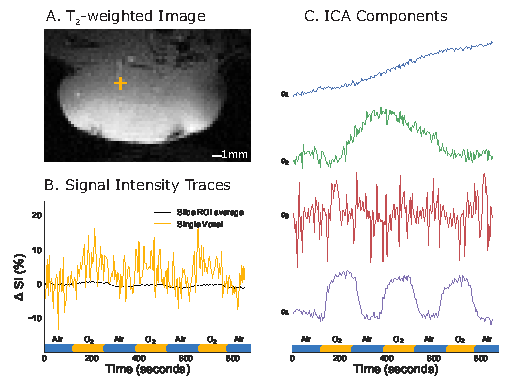
\includegraphics[width=\textwidth]{oemri_thesis1/oemri_thesis1-images/fig1_technique.pdf} % requires the graphicx package
   \caption{(A) T$_2$W MRI of a tumour xenograft at 7T and (B) the corresponding T$_1$W signal-time traces of a single voxel (solid yellow) and whole-tumour slice ROI (dotted black) during gas cycling at two-minute intervals of air (x axis; blue) and O$_2$ (x axis;yellow).
(C) Plot of the four extracted \acs{ICA} components from the entire tumour ROI, component \textbf{$c_4$} (purple) exhibits the same temporal features as the oxygen cycling time course shown along the bottom. All components are normalized, no vertical scale is shown.}
   \label{technique}
\end{figure}

\subsection{dOE-MRI with \acs{ICA} does not require assumption of a response function}
To determine whether \acs{dOE-MRI} maps obtained with a model-free \acs{ICA} approach (Figure~\ref{fig_correlation}A) are comparable to maps assuming mathematical models of the response, alternative oxygenation status correlation maps were constructed (Figure~\ref{fig_correlation}B and C). 
In Figure~\ref{fig_correlation}B and C, two example mathematical models - a square wave and the estimated hemodynamic response function (HDRF) - are correlated to the voxel-by-voxel raw time signal. 
Regions most correlated with the input paradigm remained purple in both alternative maps generated from modelled response functions.
Particularly when using the HDRF, the alternative oxygenation map showed very similar patterns in the regions demarcated as O$_2$-positive and O$_2$-negative. 
However, the map generated from correlating a square wave led to consistent underestimation of oxygenation relative to the model-free \acs{dOE-MRI} map.

\begin{figure}[htbp]
   \centering
   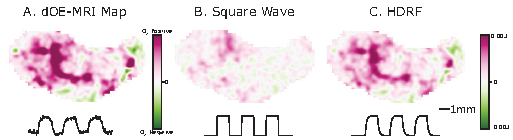
\includegraphics[width=\textwidth]{oemri_thesis1/oemri_thesis1-images/fig3_correlation.pdf} % requires the graphicx package
   \caption{(A) \acs{dOE-MRI} map of an SCCVII tumour where purple voxels contribute strongly to the extracted component using \acs{ICA} in the T$_1$W signal timecourses. 
Green voxels in the \acs{dOE-MRI} map have a strong contribution of the inverse extracted component. Pearson's r-maps are shown correlating the raw time-signal voxel by voxel with a square wave (B), and an exponential convoluted with a square wave called the hemodynamic response function (HDRF) (C).
Panels B and C are correlation maps whereas A is the \acs{dOE-MRI} map from \acs{ICA}
   \label{fig_correlation}}
\end{figure}

\subsection{Variability of response in individual oxygen cycles}

A full \acs{dOE-MRI} sequence involved three cycles of oxygen but to assess the potential for shortening the sequence we also separately applied \acs{ICA} to each of the three oxygen cycles independently.
Separate \acs{dOE-MRI} maps, as well as voxel-wise correlation plots of a representative SCCVII tumour, are shown in Figure~\ref{fig_repeatability} with Pearson's r$_{all-1}$=0.74,r$_{all-2}$=0.86,r$_{all-3}$=0.84.
Pearson's r ranged from 0.79 to 0.87 for a similar analysis in a representative HCT-116 tumour.

The stability of the independent component extraction was assessed by undersampling the full timecourse threefold prior to application of \acs{ICA}, and a high correlation between the \acs{dOE-MRI} maps from full and three-fold undersampled timecourses is observed (Figure~\ref{fig_repeatability}E; Pearson's r = 0.84). 
In Appendix~\ref{sec:interleave}, further undersampling up to a factor of six is shown with minor differences in the \acs{dOE-MRI} map.

\begin{figure}[htbp]
   \centering
   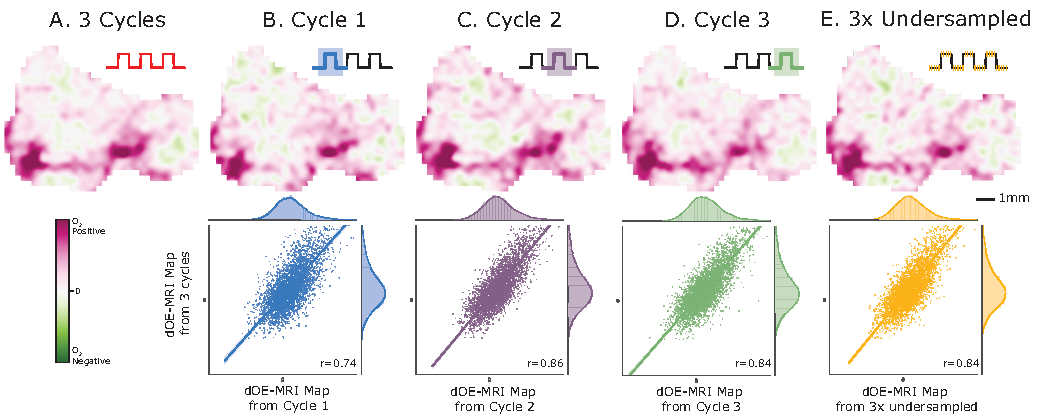
\includegraphics[width=\textwidth]{oemri_thesis1/oemri_thesis1-images/fig4_repeatability.pdf} % requires the graphicx package
   \caption{The \acs{dOE-MRI} map including the full dataset of all three cycles (A) is compared to each of the three gas cycles separately (B,C,D), and to a map that temporally undersamples by selecting every third datapoint from the full dataset (E).
Voxel-wise plots of each map are correlated to the full dataset and a linear regression with Pearson's r is shown.
   \label{fig_repeatability}}
\end{figure}

\subsection{dOE-MRI can be extended by interleaving other scans between each repetition}
\label{sec:interleave}
To investigate the subsampling limit of \acs{ICA}, Figure~\ref{subSample} shows the \acs{dOE-MRI} maps for progressively more severe undersampling.
O$_2$-positive and O$_2$-negative regions are repeatable for all maps (plot in Figure~\ref{subSample}) until subsample 5, where only 40 of the 200 available data points were used.
The original data was acquired at a temporal resolution of 4.3~s but at subsample 5, the effective temporal resolution goes to 21.3~s. 
In other words, temporal resolution could be sacrificed for \acs{SNR} simply by averaging.
More usefully, the additional time can be repurposed to interleave other scans for multi-parametric imaging within an \acs{dOE-MRI} scan.
Details of this are discussed in section~\ref{futurework:expandingdOEMRI_T2*}. 
\begin{figure}[tbhp]
   \centering
   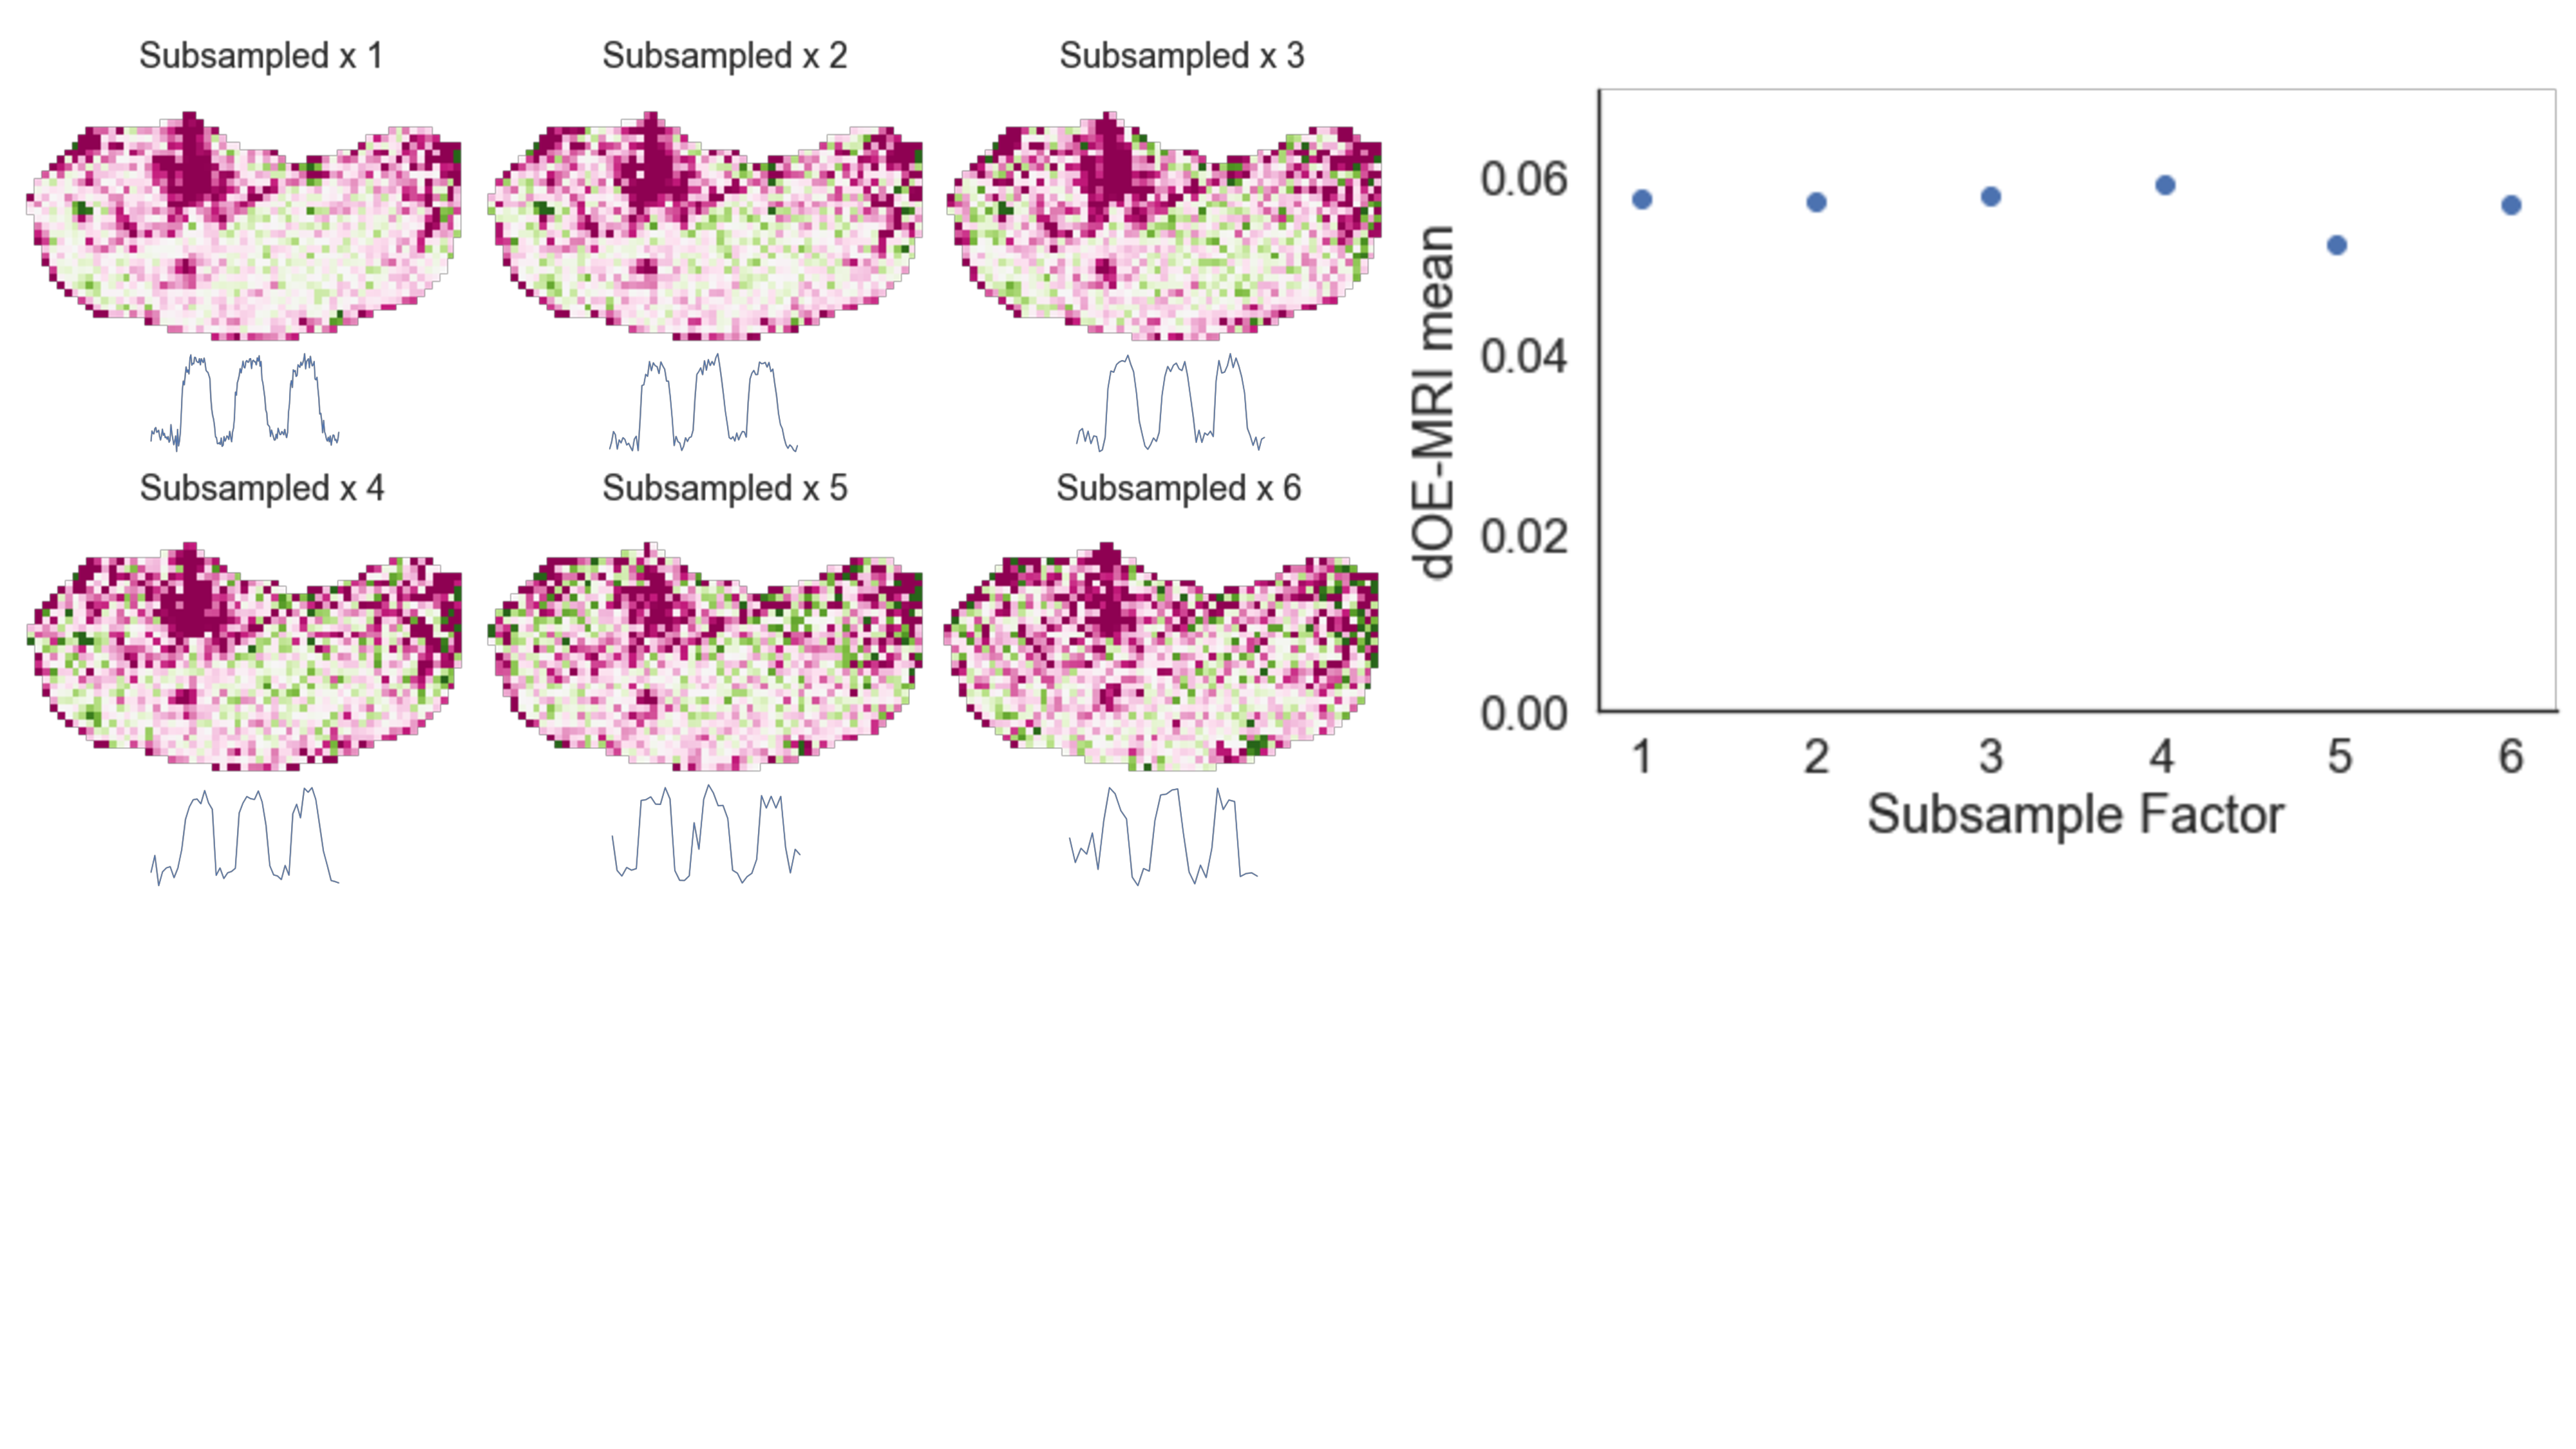
\includegraphics[width=\textwidth]{oemri_thesis1/oemri_thesis1-images/technical_subsample.pdf} % requires the graphicx package
   \caption{dOE-MRI maps and associated component traces of differently sampled data. To achieve different levels of subsampling, the raw data was spliced and then \acs{ICA} was applied. The oxygenation maps look very similar between different subsample factors. Temporal resolution and number of points were 4.3~s and 200 points (subsample 1), 8.5~s and 100 points (subsample 2), 12.8~s and 67 points (subsample 3), 17.1~s and 50 points (subsample 4), 21.3~s and 40 points (subsample 5), and 25.12~s and 34 points (subsample 6).}
   \label{subSample}
\end{figure}

\subsection{Exploring other independent components extracted using \acs{ICA}}

Figure~\ref{Sfig_components} shows the extracted independent components and their corresponding weighting factor maps for an application of \acs{ICA} on a OE-MRI scan.
Extracted components typically have a mix of high and low frequency responses and may include temperature drifts, breathing artefacts and other motion. 
For instance, c$_4$ is clearly the component of interest here as the cycling pattern is not present in any other component. 
We speculate that c$_1$ corresponds to a temperature drift over the course of the scan and c$_3$ is likely related to a breathing motion artefact. 
Component 2 is a relatively weak spurious signal fairly low in magnitude with no obvious spatial or temporal pattern. 
Additional physiological monitoring data is needed for a more thorough analysis of the other independent components and whether they can aid our understanding of the mechanism of action.

\begin{figure}[htbp]
   \centering
   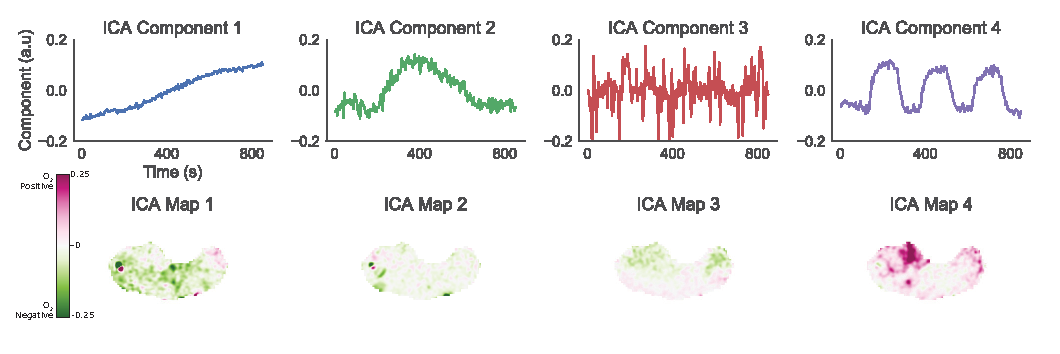
\includegraphics[width=0.9\textwidth]{oemri_thesis1/oemri_thesis1-images/fig_components.pdf} % requires the graphicx package
   \caption{Plots of the four components extracted from \acs{ICA} are shown (($||c_i||=1, \forall i $) along with the corresponding  weighting factor maps (normalized to mean voxel wise mean signal intensity).
   \label{Sfig_components}}
\end{figure}

\subsection{Comparing oxygen responsiveness with \acs{dOE-MRI} across experiments}
\label{sec:correctionfactor}
It is necessary to characterize entire tumours in a compound fashion for comparison between groups or studies. 
Existing quantification methods have involved computing fractions of positively responding and negatively responding voxels as a surrogate for oxygen responsiveness in tumours with \acs{dOE-MRI}.
However, this semi-quantitative metric relies on a binary classification of voxels as either O$_2$ positive or O$_2$-negative.
Calculating fractions is sufficient to broadly categorize tumours as oxygenated or not but consequently, rich information about the level of response is lost.
Here we present an improved quantification method of \acs{dOE-MRI} data that captures the level of response and furthermore, allows direct comparison of data acquired at varying temporal resolutions.

Since each extracted \acs{ICA} component is scaled such that its norm is one ($||c_i||=1, \forall i $), weighting factor maps are only directly comparable between scans if \acs{dOE-MRI} images are acquired at the same sampling frequency over the duration of the cycling oxygen (14 minutes).
However, holding the sampling frequency fixed over different experiments is not practical as imaging tumours of different sizes require modification of the field of view and consequently, temporal and spatial resolutions.
A scaling factor (equation~\ref{correctionfactor}; derived in the Appendix) must be applied to scale component map values so they can be compared between scans of different temporal resolutions,

\begin{equation}
s = \frac{\sqrt{N_{ref}}}{\sqrt{N}}
\label{correctionfactor}
\end{equation}

A reference sampling frequency should be chosen and in this study, it was chosen to be 0.24s$^{-1}$ (corresponding to N=198 images over the cycling oxygen).

Gas delivered to mice switches between room air and 100\% oxygen in two minute cycles, for a total of 14 minutes.
\acs{ICA} extracts the tissue response to the delivered oxygen, and four periods of room air interspersed with three periods of oxygen can be modelled mathematically using a general Heaviside function:

\begin{equation}
y(t) =
  \begin{cases}
                                   +b & \text{if $t\geq \frac{4T}{7}$} \\
                                   -b & \text{if $t< \frac{4T}{7}$} \\
  \end{cases},
\end{equation}

where $T$ is the total imaging time and $T/7$ is the time for a single segment of the gas challenge.
The Fast \acs{ICA} algorithm places a condition on the norm of the extracted component $y(t)$,

\begin{equation}
\sqrt{\sum_{i=1}^{N} \Bigl|y(t_i)\Bigr|^2} = 1.
\end{equation}

Simplifying the expression above for our $y(t)$ (the Heaviside function), we have:
\begin{align}
1 = \sqrt{b^2 \sum_{i=1}^{N} 1^2} \nonumber \\
b = N^{-\frac{1}{2}}
\end{align}

With this, we can compute the scaling factor directly using b$_{ref}$ =198 repetitions as the reference:

\begin{align}
s = \frac{b_{N}}{b_{ref}} \nonumber \\
s = \frac{\sqrt{198}}{\sqrt{N}} 
\end{align}

This scaling factor was applied to all \acs{dOE-MRI} maps used in this study to retain information about the level of response to the supplied oxygen across scans with different sampling frequencies.

%======================================================================
\section{Discussion}
% ======================================================================

In this study, we presented an improved method for OE-MRI that employs two synergistic techniques to achieve higher speed and greater sensitivity.
First, a repeated gas challenge was used to probe tissue response by introducing an independent signal modulation unrelated to nuisance contributions such as temperature drifts and motion.
A repeating gas challenge improved the detection sensitivity of small amplitude signal changes that are typical of oxygen-enhanced MRI.
Second, a repeating signal modulation enabled further improved sensitivity through the use of \acs{ICA}, a signal processing technique to isolate source signals - T$_1$W changes due solely to the cycling oxygen - without knowledge of the tissue response (Figure~\ref{technique}).
While it is possible to generate correlation maps of the oxygen cycling paradigm with T$_1$W signal changes that appear very similar to \acs{dOE-MRI} maps, an \emph{a-priori} assumption of a response function is required for this approach (Figure~\ref{fig_correlation}).
Furthermore, presupposing a particular oxygen response function biases the identification of responding O$_2$-positive voxels (Figure~\ref{fig_correlation}) underscoring the need for a model-free approach to extracting the oxygen-responding component.

The unambiguous match of the identified component with the periods of the gas cycles increases the confidence that the small T$_1$W signal changes result from increased oxygen dissolved in the plasma and interstitial tissue fluids.
Maps from other extracted components (Appendix Figure~\ref{Sfig_components}) exhibit spatial patterns that could provide clues to the signal sources but associating meaning to them is challenging and would require additional data.
For example, even moderate shifts in temperature could drive a measurable change in T$_1$W signal during the timecourse, and a physiological monitoring system that is temporally synchronized to the MR acquisition could illuminate this confounding variable. 
Nevertheless, we have established reliability of the technique by comparing maps from each cycle of the gas challenge to the map incorporating data from all three oxygen-cycles and have found no significant differences.
In fact, the strong correlations between \acs{dOE-MRI} maps from each of the individual cycles of the gas challenge (Figure~\ref{fig_repeatability}) show that it is feasible to assess tissue oxygenation within 6 minutes.
Performing this analysis again with three-fold (Figure~\ref{fig_repeatability}) and six-fold (Appendix~\ref{sec:interleave}) temporally under-sampled data suggests that there is sufficient \acs{SNR} to successfully extract the oxygen responsive component  with even a subset of the data.

dOE-MRI offers a versatile technique where the duration of the cycles and gas challenge, temporal resolution and desired signal-to-noise can be modified based on the imaging objectives, which could include investigating intermittent perfusion or intervention-mediated changes in the tumour microenvironment. 
Of note, supplying excess oxygen to hypoxic tumour cells over time has the potential for increasing the baseline oxygen concentration, effectively reducing the hypoxic fraction and altering the tumour microenvironment~\cite{Linnik:2013hf}.
This would result in voxels becoming more oxygen responsive over progressive oxygen cycles and would depend on the tumour characteristics as well as the duration of the oxygen challenge.
This was not observed on the time scales in our study when using \acs{ICA} to extract changes in T$_1$W signal intensity just due to the gas challenge. 
Should it arise in other contexts it could possibly be mitigated by extending the air-breathing part of the cycle, or by extracting that as a separate component using \acs{ICA}.
The potential for creating a hyperoxia steady state by modulating oxygen duration is discussed further by Losert et al.~\cite{Losert:2002gt}.

Depending on the application of \acs{dOE-MRI}, quantitative O$_2$-positive and O$_2$-negative fractions can be obtained from \acs{dOE-MRI} maps as shown in this study, by deploying group \acs{ICA} techniques~\cite{Calhoun:2009jr}, or setting significance thresholds using a t-test~\cite{Greicius:2004ck} and computing z-scores~\cite{McKeown:1998wd}.
In a promising study, White et al.\ has shown that OE-MRI may be very relevant in developing prognostic factors to predict tumour response to hypofractionation by stratifying tumours that may benefit from oxygen breathing during irradiation~\cite{White:2016fz}.
Featherstone et al.\ have recently explored pre-clinical datasets using feature-extraction and clustering analysis and this may prove fruitful in understanding the behavior of subregions within a tumour microenvironment~\cite{Featherstone:2018cn}.
Future work to evaluate the utility of \acs{dOE-MRI} will ultimately depend on its context-dependent validation as a relevant measure of tumour hypoxia to dynamically characterize the clinically relevant oxygen status of tumours, relating this information to treatment sensitivities and outcomes.

% ======================================================================
\section{Conclusions}
% ======================================================================
In this study we extend existing oxygen-enhanced MRI techniques by adding a cycling element to the respiratory challenge and using a blind-source separation signal processing technique (\acs{ICA}) to extract the oxygen responsive component and responding voxels.
In the following chapters, we advance development and application of the technique and further refine it. 
In chapter~\ref{ch:oemri2} we attempt to validate \acs{dOE-MRI} measurements \emph{in vivo} using pimonidazole, a histological tumour hypoxia marker.
To further explore the oxygen dynamics in tumours we also characterized the oxygen replenishment curve as originally proposed by Losert et al.\ in the brain~\cite{Losert:2002gt}.
In chapter~\ref{ch:oemri3} we deploy the technique to assess tumour oxygenation changes following treatment with bevacizumab, an antiangiogenic agent.

\endinput
